 \documentclass[conference]{IEEEtran}
\IEEEoverridecommandlockouts
% The preceding line is only needed to identify funding in the first footnote. If that is unneeded, please comment it out.
\usepackage{cite}
\usepackage{amsmath,amssymb,amsfonts}
\usepackage{algorithmic}
\usepackage{graphicx}
\usepackage{float} 
\usepackage{subfigure} 
\usepackage{textcomp}
\usepackage{xcolor}
\def\BibTeX{{\rm B\kern-.05em{\sc i\kern-.025em b}\kern-.08em
    T\kern-.1667em\lower.7ex\hbox{E}\kern-.125emX}}
\begin{document}

\title{Software Specification: Tripedia\\
}

\author{\IEEEauthorblockN{Yulin Zhang}
\IEEEauthorblockA{\textit{7th Group} \\
\textit{Software Engineering}\\
Montreal, Canada \\
silveralex2023820@gmail.com}
\and
\IEEEauthorblockN{Yuhang Chen}
\IEEEauthorblockA{\textit{7th Group} \\
\textit{Software Engineering}\\
Montreal, Canada \\
yuhang.chen@mail.concordia.ca}
\and
\IEEEauthorblockN{Jiaxi Yang}
\IEEEauthorblockA{\textit{7th Group} \\
\textit{Software Engineering}\\
Montreal, Canada \\
yjxyang2@outlook.com}
\and
\IEEEauthorblockN{Boyang Wang}
\IEEEauthorblockA{\textit{7th Group} \\
\textit{Software Engineering}\\
Montreal, Canada \\
wangboyang0626@outlook.com}
}

\maketitle


\begin{figure*}[htbp]
\centerline{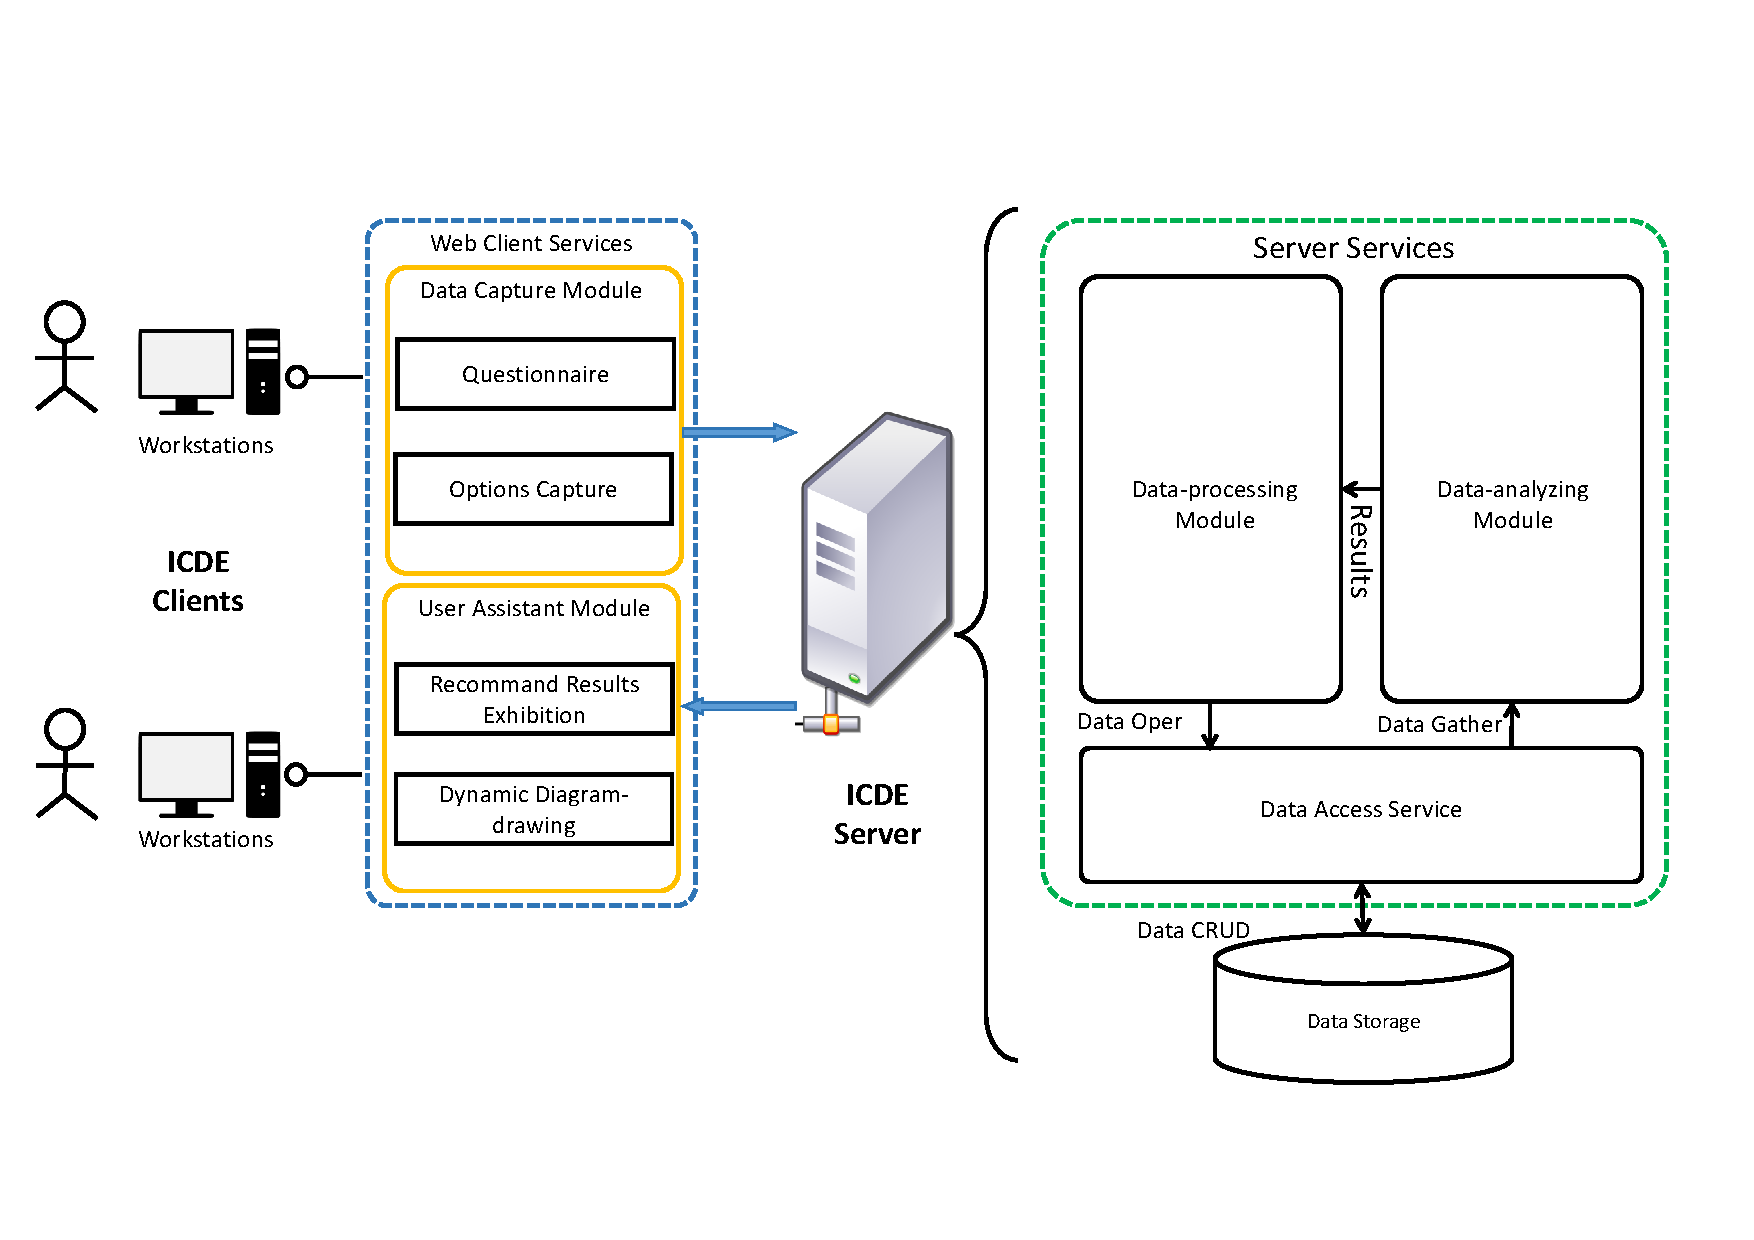
\includegraphics[width=0.9\textwidth]{Architecture.pdf}}
\caption{The architecture graph of Tripedia.}
\label{fig1}
\end{figure*}

\section{Introduction}


\subsection{Problem Statement}

Travel has gradually become an indispensable part of people's lives. According to relevant research, 83\% of Canadians will travel to different cities to experience different customs during their holidays. Travel planning has become a problem that troubles most Canadians. At the same time, many people don’t know which places are more suitable for them. Therefore, travel recommendations and planning have become essential issues affecting people's quality of life.


\subsection{Architecture Design}

As shown in Figure\ref{fig1}, the ICDE system architecture mainly contains two parts: client and server. Based on the limited server hardware equipment, we implement the data analysis logic as a single module in the server, which stands for ICDE 3rd Party Applications. 

In the client part, we implement Tripedia's client logic based on the web. The web client service is mainly divided into two parts: the Data Capture Module and User Assistant Module. The Data Capture Module captures the user's behavior and personal information through questionnaires and behavior captures, and transmits the relevant information to the server. The User Assistant Module is responsible for displaying processed data sent by the server, such as recommendation results and data analysis results, which help users make decisions easily.

On the server side, we will develop three modules to implement the backbone of the ICDE system: Data-processing Module, Data-analyzing Module, and Data Access Service. The Data Access Service, as the median layer for database access, provides a unified database interface (deletion, modification, query, etc) for the Data-processing Module and the Data-analyzing module. The Data-processing Module is responsible for the basic logic of the server, such as registration, login, search, data preprocessing, and other interaction logic with the client. The Data-analyzing Module accesses the data in the database through the Data Access Service to perform data analysis and returns the analysis results to the Data-processing Module.

To sum up, Tripedia's architecture is a standard ICDE system. The Client part includes a Data Capture Service to collect user behavior and information and transmit relevant data to the server. The Data-processing Module in the Servers section is responsible for implementing the interactive logic of the server; the Data Access Service provides a unified data access interface; the Data-analyzing Module serves as the core of the ICDE system to analyze user data and feedback the analysis results to the user through the server to provide User Assistance Service.

\section{Overview}



\subsection{Project Goal}

The goal of the project is to solve the travel planning difficulties faced by users. In response to travel planning issues, this project set out to develop search features to help users. Meanwhile, some users don’t know where is more suitable for travel. This project provides clear charts through the background data analysis function to help users make better decisions. 

\subsection{Key Functionalities}

\textbf{Search} The search feature is responsible for obtaining search results based on the user's search keywords and collected user preferences. This function includes searching for tourist cities, searching for hotels, etc. The search function can provide users with travel route planning.

\textbf{Data Analysis}If the user doesn't know where is better for vacation, the website provides a data analysis function. Based on current user preferences and existing data in the system, the website provides data analysis charts of tourist cities suitable for users to help users make better decisions.

\subsection{User Stories}


1. The traveler opens the travel website without logging in, the website will collect his location, so that the website can show local people's favorite place to visit which provides a reference for the user.

2. The traveler registers an account and login to the Tripedia website.

3. The traveler finishes a questionnaire so that the website can recommend appropriate information for users based on the questionnaire content.

4. The traveler has no idea about the where is the best places for him. He finds the data analysis diagram panel for more information to make a decision.

5. The traveler searches for his destination and then the website recommends related information (e.t. hotel, transport function, Landmark Tickets, scenic spot review) so that he can make plans by reference.

6. The traveler checks suitable hotel timings so that he can book an appropriate hotel.

7. The traveler checks suitable flight or train timing so that he can book an appropriate transport function.

8. The traveler selects his favorite hotel and then clicks to jump to the booking screen so that he can make payment.



\subsection{User Cases}


\subsubsection{User Cases: Open Website}

\textbf{ }

\textbf{Use Case}: Open Website without Login.

\textbf{Actors}: Traveller, Client, Server, Analysis Module.

\textbf{Summary Description}:Allows any travelers to open Tripedia, and Tripedia shows some basic information about traveling according to the traveler's position.
 
\textbf{Status}: Medium level of details.

\textbf{Pre-condition}: Traveler has to register an account and log in to the Tripedia website to use its service.

\textbf{Post-condition}: The traveler has to have a personal computer and an available network environment.

\textbf{Basic-Path}:

1. The traveler enters the Tripedia website in a browser.

2. The Tripedia website catches the user's position and sends the basic information to the server.

3. The server recommends the travel information entry based on the user's position.

4. The website displays the available travel information sent by the server.

\textbf{Alternate Paths}:

None.

\subsubsection{User Cases: Register and Login}

\textbf{ }

\textbf{Use Case}: Register

\textbf{Actors}: Traveller, Client, Server, Data Store.

\textbf{Summary Description}: Allows any traveller register an account and login in the Tripedia website.
 
\textbf{Status}: Medium level of details.

\textbf{Pre-condition}: The traveler has to open the Tripedia website without login.

\textbf{Post-condition}: Traveler has to complete the questionnaire to use Tripedia's full service.

\textbf{Basic-Path}:

1. The traveler clicks the "register" button on the home page and enters the register page.

2. The traveler fills in the register information: user name, nationality, gender, and password. Then the traveler clicks the "submit" button.

3. The server validates the username is repetitive in the system, and saves the register information to Data Store.

4. The client displays the "register successfully" information and enters the login page.

5. The traveler fills in the user information: user name, and password. The the traveller clicks "login" button.

6. The server recommends the travel information entry based on the user's information and transfers the recommended information to the client.

7. The client enters the home page and displays the information entry sent by the server.

\textbf{Alternate Paths}:

3a. The user name is repetitive in the system.

5a. The user forgets username/password.


\subsubsection{User Cases: Questionnaire}

\textbf{ }

\textbf{Use Case}: Questionnaire

\textbf{Actors}: Traveller, Client, Server, Data Store.

\textbf{Summary Description}: Allows any traveler within the login state to have opportunities to complete the questionnaire to get appropriate recommendations.
 
\textbf{Status}: Medium level of details.

\textbf{Pre-condition}: Traveler must be in login state.

\textbf{Post-condition}: None

\textbf{Basic-Path}:

1. The traveler logs in to the website firstly, the website pops up a dialog to ask the user to fill out a questionnaire.

2. The traveler clicks "yes", and the client enters the questionnaire page.

3. The website has several questions about preference. The traveler can select one answer for each question.

4. The traveler clicks the "submit" button, and the answers are sent to the server.

5. The server recommends the travel information entry based on the user's answers and transfers the recommended information to the client.

7. The client enters the home page and displays the information entry sent by the server.

\textbf{Alternate Paths}:

2a. The user abandons the chance to complete the questionnaire.




\subsubsection{User Cases: Data Analysis Diagram}

\textbf{ }

\textbf{Use Case}: Questionnaire

\textbf{Actors}: Traveller, Client, Server.

\textbf{Summary Description}: Allows any traveler within the login state to check the data analysis diagram.
 
\textbf{Status}: Medium level of details.

\textbf{Pre-condition}: Travelers must be in login state and the website is on home page.

\textbf{Post-condition}: Travelers can search the recommended cities in the search area for more information.

\textbf{Basic-Path}:


1. The traveler clicks the "Analysis Panel" button.

2. The client enters the Data Analysis Page.

3. The server sends the analyzed data based on the user's information to the client.

4. The website displays the diagrams of recommended cities, such as the visitors' number, the visitors' nationalities proportion, etc.

\textbf{Alternate Paths}: None.





\section{Functional Requirements}



\section{Unfunctional Requirements}




\end{document}
